Nguồn: \href{https://tiasang.com.vn/khoa-hoc-cong-nghe/Viet-ve-anh-giao-su-Phan-Dinh-Dieu-12393}{Báo Tia Sáng}

\begin{figure}
\centering
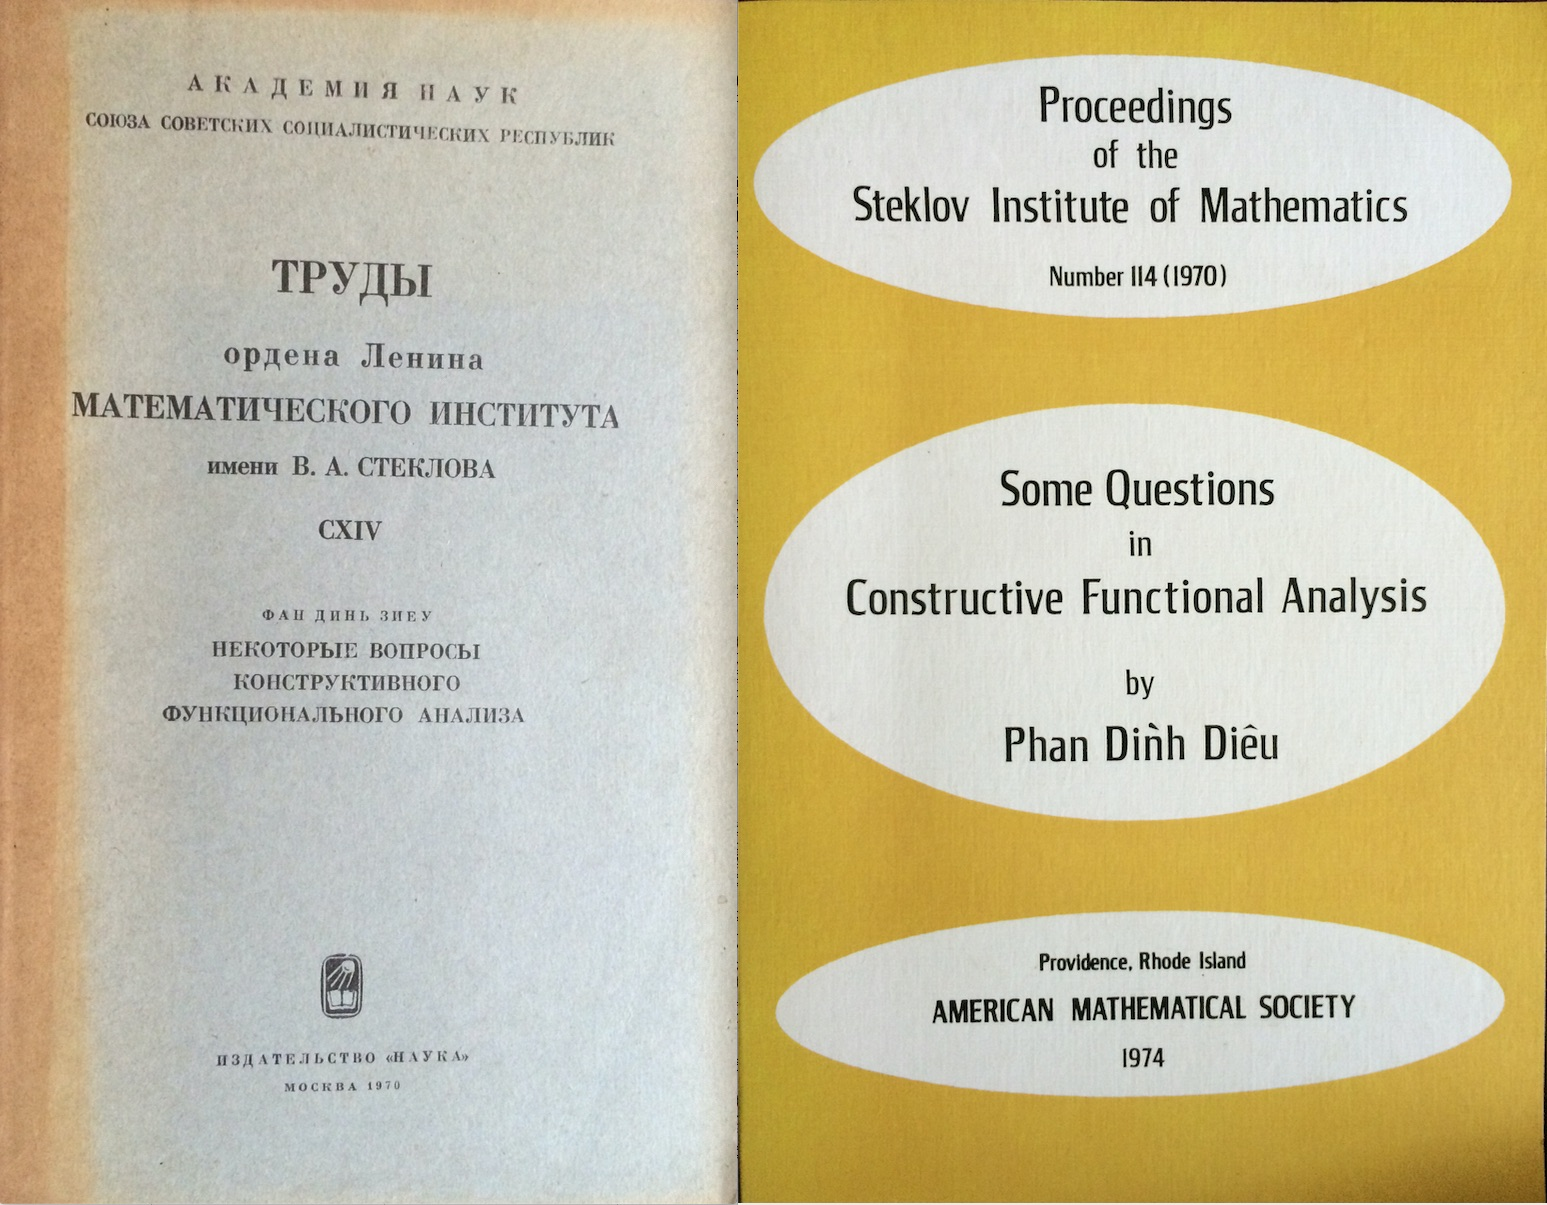
\includegraphics[scale=0.12]{Photos/DieuThesis}
\caption{Công trình về \textit{Giải tích hàm kiến thiết} của GS Phan Đình Diệu được in thành sách của Steklov Institute of Mathematics và sau đó được dịch sang tiếng Anh bởi American Mathematical Society. Xem thêm bài viết của GS Lê Tự Quốc Thắng ở phần \ref{LTQT} }
\end{figure}
Thế là Anh đã ra đi.

Mấy hôm nay trên báo chí, trên “cộng đồng mạng” tràn ngập những bài viết, những lời bày tỏ tình cảm với Anh. Ai cũng muốn viết gì đó về Anh.

Tôi cũng vậy.

Nhưng viết về Anh thật khó. Không thể nói những lời thừa. Không thể nói những lời mọi người đều đã nói. Con người Anh luôn độc đáo, sâu sắc, chính xác. Rất khó bỏ đi dù chỉ một từ nào đó trong những bài viết của Anh.

Anh độc đáo ngay từ khi chập chững vào làng Toán. Vì thích Số học mà Anh đã tự học tiếng Trung để dịch cuốn Số học của Hoa La Canh. Vì yêu thích sự chính xác mà anh chọn cho mình môn Logic khi đi làm nghiên cứu sinh ở Liên Xô. Chỉ trong 5 năm, anh đã xây dựng nên một ngành mới trong Toán học: Giải tích hàm kiến thiết. Công trình của anh được in thành sách (Some questions in constructive functional analysis. Proceedings of the Steklov Institute of Mathematics, No. 114 (1970). Translated from the Russian by J. M. Danskin.American Mathematical Society, Providence, R.I., 1974. iv+228 pp.). Chữ “kiến thiết” được dùng cho những ngành Toán mà ở đó không chấp nhận chứng minh phản chứng: không thể khẳng định một cái gì đó là “tồn tại” nếu điều giả thiết “nó không tồn tại” dẫn đến nghịch lý. Muốn chứng minh “tồn tại”, phải đưa ra thuật toán xây dựng (“kiến thiết”) nó.

Tư tưởng “kiến thiết” đó cũng làm Anh trở nên gần gũi với Khoa học máy tính một cách tự nhiên. Và với nhãn quan sáng suốt của mình, Anh nhận ra ngay từ những năm đầu của thập ký 70, thế kỷ trước, rằng Tin học chính là Khoa học của tương lai, và Việt Nam nhất thiết phải xây dựng ngành Tin học. Có thể nói rằng trình độ Tin học của Việt Nam thời kỳ đó cao hơn nếu so sánh với những nước trong vùng Đông Nam Á. Chúng ta đã từng đi trước, nhưng vì nhiều nguyên nhân nên đã tụt lại phía sau.

Đọc lại những bài viết của Anh về Khoa học, về con đường phát triển của xã hội Việt Nam, không thể không ngạc nhiên về những kiến giải sâu sắc, độc đáo, về tầm nhìn của anh. Sự phát triển, những vấn đề mà xã hội đang phải đối mặt gần như là “minh hoạ” những gì Anh nói đã vài chục năm. Và trên hết, ta cảm nhận tấm lòng Anh, một kẻ sỹ của thời đại mới, luôn trăn trở với con đường đi của đất nước.

Anh không chỉ là nhà khoa học, nhà tư tưởng, Anh là người say mê tất cả những gì thuộc về tri thức nhân loại. Tôi còn nhớ, Anh đã bình rất hay về cảnh đối đáp giữa Khuất Nguyên và Ngư Phủ trên sông Tương (trong một bài viết, hình như đăng trên báo Văn Nghệ). Những lần trò chuyện về Thơ, tôi thấy Anh rất thích Rabindranath Tagore, đặc biệt là những câu:

Đôi mắt lo âu của em buồn,\\
đôi mắt em muốn tìm vào tâm tưởng của anh\\
như trăng kia muốn vào sâu biển cả…\\

Trái tim anh cũng ở gần em,\\
như chính cuộc đời của em vậy\\
nhưng chẳng bao giờ em hiểu hết nó đâu.\\

Hình như Anh luôn có cảm giác người khác không hiểu hết mình. Mà đúng vậy. Anh sâu sắc quá, độc đáo quá, nghĩ xa hơn người khác nhiều quá, để người ta có thể hiểu hết về Anh. Nhưng dù không hiểu hết, Anh vẫn chiếm trọn tình yêu và lòng khâm phục của những người có dịp gần Anh.

Những lời sau đây của Tagore viết về Cái Chết, hình như cũng chính là dành cho Anh:

Khi nghĩ về những năm tháng đã qua,\\
đã trôi xuôi theo theo giòng chảy\\
của cuộc sống, và tình yêu, và cái chết,\\
tôi thấy sự ra đi vĩnh viễn là tự do biết bao.\\

Không cần phải nói lời cầu mong Anh yên nghỉ. Dường như Anh đã đi xa, để có thể được tự do suy tưởng. Một mình.
